\documentclass[11pt, letterpaper]{article}

% Fonts and Encoding
\usepackage[utf8]{inputenc}
\usepackage[T1]{fontenc}
\usepackage{lmodern} % High-quality Latin Modern vector font

% Math and Symbols
\usepackage{amsmath, amssymb, amsthm, amsfonts, mathrsfs, mathtools}

% Layout and Geometry
\usepackage{geometry}
\geometry{letterpaper, margin=1in}
\setlength{\parindent}{0pt}
\setlength{\parskip}{0.6em}

% Formatting and Graphics
\usepackage{graphicx, xcolor, enumitem, booktabs, array, tabularx}

% TikZ for Illustrations
\usepackage{tikz}
\usetikzlibrary{arrows.meta, positioning, shapes.geometric, calc, backgrounds, matrix}

% Clickable Links and TOC
\usepackage{hyperref}
\hypersetup{
    colorlinks=true,
    linkcolor=blue,
    filecolor=magenta,      
    urlcolor=cyan,
    pdftitle={Advanced Mathematics Topic},
}

% Theorem Environments
\newtheorem{theorem}{Theorem}[section]
\newtheorem{lemma}[theorem]{Lemma}
\newtheorem{proposition}[theorem]{Proposition}
\newtheorem{corollary}[theorem]{Corollary}
\theoremstyle{definition}
\newtheorem{definition}{Definition}[section]
\newtheorem{axiom}{Axiom}[section]
\newtheorem{example}{Example}[section]
\theoremstyle{remark}
\newtheorem{remark}{Remark}[section]

% Custom Commands (Enforced standard notation)
\newcommand{\R}{\mathbb{R}}
\newcommand{\N}{\mathbb{N}}
\newcommand{\Z}{\mathbb{Z}}
\newcommand{\Q}{\mathbb{Q}}
\newcommand{\E}{\mathbb{E}}
\newcommand{\Prob}{\mathbb{P}}
\newcommand{\F}{\mathcal{F}}

\begin{document}

\title{\textbf{Advanced Mathematics: Power Series and Analytic Functions}}
\author{Tashfeen Omran}
\date{\today}
\maketitle

\tableofcontents
\newpage

\section{Part 1: Comprehensive Introduction, Context, and Prerequisites}

\subsection{Core Concepts}
A \textbf{power series} about a point $x_0$ is an infinite series of the form:
\[ \sum_{n=0}^{\infty} a_n (x - x_0)^n = a_0 + a_1(x - x_0) + a_2(x - x_0)^2 + \cdots \]
where $x$ is a variable and $a_n$ are constant coefficients. The central question regarding any power series is its \textbf{convergence}: for which values of $x$ does this infinite sum evaluate to a finite real number? 

Every power series has a \textbf{radius of convergence}, denoted $\rho$ (or $R$). The series converges absolutely for $|x - x_0| < \rho$ and diverges for $|x - x_0| > \rho$. The behavior at the exact boundary points $x = x_0 \pm \rho$ must be checked manually. A function $f(x)$ is called \textbf{analytic} at $x_0$ if it can be represented by a power series with a positive radius of convergence in some neighborhood of $x_0$.

\subsection{Intuition and Derivation}
The intuition behind power series is the desire to represent complex, non-algebraic functions (like $e^x$, $\sin x$, $\ln x$) as "infinite polynomials." Polynomials are mathematically "nice"—they are easy to evaluate, differentiate, and integrate. By extending a polynomial to an infinite degree, we can perfectly match the behavior of smooth functions. The coefficients $a_n$ are derived by matching the derivatives of the series to the derivatives of the function at the center $x_0$, leading to the \textbf{Taylor Series} formula: $a_n = \frac{f^{(n)}(x_0)}{n!}$.

\subsection{Historical Context and Motivation}
In the 17th and 18th centuries, mathematicians like Isaac Newton, Brook Taylor, and Colin Maclaurin sought methods to compute values of transcendental functions and solve complex differential equations. Newton used infinite series to integrate functions that had no known antiderivatives. The formalization of Taylor series allowed mathematicians to transform differential equations (which involve unknown functions and their derivatives) into algebraic equations involving the coefficients $a_n$, birthing the \textbf{Power Series Method} for solving differential equations.

\subsection{Key Formulas}
\begin{itemize}
    \item \textbf{Taylor Series:} $f(x) = \sum_{n=0}^{\infty} \frac{f^{(n)}(x_0)}{n!} (x - x_0)^n$
    \item \textbf{Maclaurin Series:} A Taylor series centered at $x_0 = 0$.
    \item \textbf{Ratio Test for Radius of Convergence:} $\rho = \lim_{n \to \infty} \left| \frac{a_n}{a_{n+1}} \right|$ (if the limit exists).
    \item \textbf{Cauchy Product:} $\left(\sum_{n=0}^{\infty} a_n x^n\right) \left(\sum_{n=0}^{\infty} b_n x^n\right) = \sum_{n=0}^{\infty} c_n x^n$, where $c_n = \sum_{k=0}^{n} a_k b_{n-k}$.
\end{itemize}

\subsection{Prerequisites}
To master this topic, you must be proficient in:
1. \textbf{Infinite Series Tests:} Specifically the Ratio Test, Alternating Series Test, and $p$-series test.
2. \textbf{Calculus I \& II:} Strong differentiation and integration skills, including the Chain Rule and L'H\^{o}pital's Rule.
3. \textbf{Algebraic Manipulation:} Factoring, expanding polynomials, and shifting summation indices (e.g., changing variables from $n$ to $k$).

\newpage
\section{Part 2: Detailed Homework Solutions}

\subsection{Problems 1--6: Determine the Convergence Set}

\textbf{Problem 1:} $\displaystyle \sum_{n=0}^{\infty} \frac{2^{-n}}{n+1} (x-1)^n$
\\[6pt]
\textbf{Solution:} We apply the Ratio Test. Let $c_n = \frac{2^{-n}}{n+1} (x-1)^n$.
\[ \lim_{n \to \infty} \left| \frac{c_{n+1}}{c_n} \right| = \lim_{n \to \infty} \left| \frac{2^{-(n+1)}(x-1)^{n+1}}{n+2} \cdot \frac{n+1}{2^{-n}(x-1)^n} \right| = \lim_{n \to \infty} \frac{1}{2} \frac{n+1}{n+2} |x-1| = \frac{|x-1|}{2} \]
For convergence, we require $\frac{|x-1|}{2} < 1 \implies |x-1| < 2$. The radius of convergence is $\rho = 2$. The open interval is $-1 < x < 3$.
Check endpoints:
At $x = 3$: $\sum_{n=0}^{\infty} \frac{2^{-n}}{n+1} (2)^n = \sum_{n=0}^{\infty} \frac{1}{n+1}$, which is the harmonic series (diverges).
At $x = -1$: $\sum_{n=0}^{\infty} \frac{2^{-n}}{n+1} (-2)^n = \sum_{n=0}^{\infty} \frac{(-1)^n}{n+1}$, which is the alternating harmonic series (converges).
\textbf{Final Answer:} $[-1, 3)$

\textbf{Problem 2:} $\displaystyle \sum_{n=0}^{\infty} \frac{3^n}{n!} x^n$
\\[6pt]
\textbf{Solution:} Let $c_n = \frac{3^n}{n!} x^n$.
\[ \lim_{n \to \infty} \left| \frac{c_{n+1}}{c_n} \right| = \lim_{n \to \infty} \left| \frac{3^{n+1} x^{n+1}}{(n+1)!} \cdot \frac{n!}{3^n x^n} \right| = \lim_{n \to \infty} \frac{3 |x|}{n+1} = 0 \]
Since $0 < 1$ for all $x \in \R$, the series converges everywhere.
\textbf{Final Answer:} $(-\infty, \infty)$

\textbf{Problem 3:} $\displaystyle \sum_{n=0}^{\infty} \frac{n^2}{2^n} (x+2)^n$
\\[6pt]
\textbf{Solution:} Let $c_n = \frac{n^2}{2^n} (x+2)^n$.
\[ \lim_{n \to \infty} \left| \frac{c_{n+1}}{c_n} \right| = \lim_{n \to \infty} \left| \frac{(n+1)^2 (x+2)^{n+1}}{2^{n+1}} \cdot \frac{2^n}{n^2 (x+2)^n} \right| = \lim_{n \to \infty} \frac{1}{2} \left(\frac{n+1}{n}\right)^2 |x+2| = \frac{|x+2|}{2} \]
Convergence requires $\frac{|x+2|}{2} < 1 \implies |x+2| < 2$. The open interval is $-4 < x < 0$.
Check endpoints:
At $x = 0$: $\sum_{n=0}^{\infty} n^2$, which diverges by the $n$-th term test.
At $x = -4$: $\sum_{n=0}^{\infty} (-1)^n n^2$, which diverges by the $n$-th term test.
\textbf{Final Answer:} $(-4, 0)$

\textbf{Problem 4:} $\displaystyle \sum_{n=1}^{\infty} \frac{4}{n^2+2n} (x-3)^n$
\\[6pt]
\textbf{Solution:} Let $c_n = \frac{4}{n^2+2n} (x-3)^n$.
\[ \lim_{n \to \infty} \left| \frac{c_{n+1}}{c_n} \right| = \lim_{n \to \infty} \left| \frac{4(x-3)^{n+1}}{(n+1)^2+2(n+1)} \cdot \frac{n^2+2n}{4(x-3)^n} \right| = |x-3| \lim_{n \to \infty} \frac{n^2+2n}{n^2+4n+3} = |x-3| \]
Convergence requires $|x-3| < 1 \implies 2 < x < 4$.
Check endpoints:
At $x = 4$: $\sum_{n=1}^{\infty} \frac{4}{n^2+2n}$. Since $\frac{4}{n^2+2n} \sim \frac{4}{n^2}$, it converges by limit comparison to a $p$-series ($p=2 > 1$).
At $x = 2$: $\sum_{n=1}^{\infty} \frac{4(-1)^n}{n^2+2n}$. Converges absolutely.
\textbf{Final Answer:} $[2, 4]$

\textbf{Problem 5:} $\displaystyle \sum_{n=1}^{\infty} \frac{3}{n^3} (x-2)^n$
\\[6pt]
\textbf{Solution:} Let $c_n = \frac{3}{n^3} (x-2)^n$.
\[ \lim_{n \to \infty} \left| \frac{c_{n+1}}{c_n} \right| = \lim_{n \to \infty} \left| \frac{3(x-2)^{n+1}}{(n+1)^3} \cdot \frac{n^3}{3(x-2)^n} \right| = |x-2| \lim_{n \to \infty} \left(\frac{n}{n+1}\right)^3 = |x-2| \]
Convergence requires $|x-2| < 1 \implies 1 < x < 3$.
Check endpoints:
At $x = 3$: $\sum_{n=1}^{\infty} \frac{3}{n^3}$, converges ($p$-series, $p=3 > 1$).
At $x = 1$: $\sum_{n=1}^{\infty} \frac{3(-1)^n}{n^3}$, converges absolutely.
\textbf{Final Answer:} $[1, 3]$

\textbf{Problem 6:} $\displaystyle \sum_{n=0}^{\infty} \frac{(n+2)!}{n!} (x+2)^n$
\\[6pt]
\textbf{Solution:} Simplify the coefficients: $\frac{(n+2)!}{n!} = (n+2)(n+1)$. The series is $\sum_{n=0}^{\infty} (n+2)(n+1)(x+2)^n$.
\[ \lim_{n \to \infty} \left| \frac{c_{n+1}}{c_n} \right| = \lim_{n \to \infty} \left| \frac{(n+3)(n+2)(x+2)^{n+1}}{(n+2)(n+1)(x+2)^n} \right| = |x+2| \lim_{n \to \infty} \frac{n+3}{n+1} = |x+2| \]
Convergence requires $|x+2| < 1 \implies -3 < x < -1$.
Check endpoints:
At $x = -1$: $\sum_{n=0}^{\infty} (n+2)(n+1)$, diverges ($n$-th term test).
At $x = -3$: $\sum_{n=0}^{\infty} (-1)^n(n+2)(n+1)$, diverges.
\textbf{Final Answer:} $(-3, -1)$

\subsection{Problem 7: Ratio Test for Zero-Pattern Series}
\textbf{Problem 7:} Show that $\sum_{k=0}^{\infty} a_{2k} x^{2k}$ has radius of convergence $\rho = \frac{1}{\sqrt{L}}$ if $\lim_{k \to \infty} \left| \frac{a_{2k+2}}{a_{2k}} \right| = L$.
\\[6pt]
\textbf{Solution:} Let $z = x^2$. The series becomes $\sum_{k=0}^{\infty} a_{2k} z^k$. Applying the standard Ratio Test for the variable $z$:
\[ \lim_{k \to \infty} \left| \frac{a_{2k+2} z^{k+1}}{a_{2k} z^k} \right| = |z| \lim_{k \to \infty} \left| \frac{a_{2k+2}}{a_{2k}} \right| = L |z| \]
For convergence, we need $L |z| < 1 \implies |z| < \frac{1}{L}$. Substituting back $z = x^2$, we get $|x^2| < \frac{1}{L} \implies |x| < \frac{1}{\sqrt{L}}$. Thus, $\rho = \frac{1}{\sqrt{L}}$.
For the odd series $\sum_{k=0}^{\infty} a_{2k+1} x^{2k+1} = x \sum_{k=0}^{\infty} a_{2k+1} x^{2k}$, let $z = x^2$. The limit is $M |z| < 1 \implies |x| < \frac{1}{\sqrt{M}}$. Thus $\rho = \frac{1}{\sqrt{M}}$.

\subsection{Problem 8: Determine Convergence Sets}
\textbf{Solution:}
(a) $\sum_{k=0}^{\infty} 2^{2k} x^{2k}$. Let $a_{2k} = 2^{2k}$. $\lim \left| \frac{a_{2k+2}}{a_{2k}} \right| = \frac{2^{2k+2}}{2^{2k}} = 4 = L$. By Problem 7, $\rho = \frac{1}{\sqrt{4}} = \frac{1}{2}$. Endpoints $x = \pm \frac{1}{2}$ yield $\sum 1$, which diverges. \textbf{Set:} $(-\frac{1}{2}, \frac{1}{2})$.
\\[4pt]
(b) $\sum_{k=0}^{\infty} 2^{2k+1} x^{2k+1}$. $a_{2k+1} = 2^{2k+1}$. $\lim \left| \frac{a_{2k+3}}{a_{2k+1}} \right| = 4 = M$. $\rho = \frac{1}{2}$. Endpoints diverge. \textbf{Set:} $(-\frac{1}{2}, \frac{1}{2})$.
\\[4pt]
(c) $\sin x = \sum_{n=0}^{\infty} \frac{(-1)^n}{(2n+1)!} x^{2n+1}$. $a_{2n+1} = \frac{(-1)^n}{(2n+1)!}$. $\lim \left| \frac{a_{2n+3}}{a_{2n+1}} \right| = \lim \frac{(2n+1)!}{(2n+3)!} = \lim \frac{1}{(2n+2)(2n+3)} = 0$. $\rho = \infty$. \textbf{Set:} $(-\infty, \infty)$.
\\[4pt]
(d) $\cos x$. Similar to (c), the limit of the ratio of coefficients is 0. $\rho = \infty$. \textbf{Set:} $(-\infty, \infty)$.
\\[4pt]
(e) $(\sin x)/x = \sum_{n=0}^{\infty} \frac{(-1)^n}{(2n+1)!} x^{2n}$. The coefficients are the same as in (c). $\rho = \infty$. \textbf{Set:} $(-\infty, \infty)$.
\\[4pt]
(f) $\sum_{k=0}^{\infty} 2^{2k} x^{4k}$. Let $z = x^4$. Series is $\sum 2^{2k} z^k$. Ratio test: $\lim \frac{2^{2k+2}}{2^{2k}} = 4$. Converges for $|z| < \frac{1}{4} \implies |x^4| < \frac{1}{4} \implies |x| < \frac{1}{\sqrt{2}}$. Endpoints diverge. \textbf{Set:} $(-\frac{1}{\sqrt{2}}, \frac{1}{\sqrt{2}})$.

\subsection{Problems 9--10: Power Series Expansion for Sums}
\textbf{Problem 9:} $f(x) = \sum_{n=0}^{\infty} \frac{1}{n+1} x^n$, $g(x) = \sum_{n=1}^{\infty} 2^{-n} x^{n-1}$. Find $f(x) + g(x)$.
\\[6pt]
\textbf{Solution:} First, shift the index of $g(x)$ to match the $x^n$ term. Let $k = n-1 \implies n = k+1$.
\[ g(x) = \sum_{k=0}^{\infty} 2^{-(k+1)} x^k = \sum_{n=0}^{\infty} 2^{-(n+1)} x^n \]
Now add term-by-term:
\[ f(x) + g(x) = \sum_{n=0}^{\infty} \left( \frac{1}{n+1} + \frac{1}{2^{n+1}} \right) x^n \]

\textbf{Problem 10:} $f(x) = \sum_{n=3}^{\infty} \frac{2^n}{n!} (x-1)^{n-2}$, $g(x) = \sum_{n=1}^{\infty} \frac{n^2}{2^n} (x-1)^{n-1}$.
\\[6pt]
\textbf{Solution:} Shift indices to get $(x-1)^k$.
For $f(x)$, let $k = n-2 \implies n = k+2$. The sum starts at $k=1$: $f(x) = \sum_{k=1}^{\infty} \frac{2^{k+2}}{(k+2)!} (x-1)^k$.
For $g(x)$, let $k = n-1 \implies n = k+1$. The sum starts at $k=0$: $g(x) = \sum_{k=0}^{\infty} \frac{(k+1)^2}{2^{k+1}} (x-1)^k$.
Isolate the $k=0$ term from $g(x)$: $g_0 = \frac{1^2}{2^1} = \frac{1}{2}$.
\[ f(x) + g(x) = \frac{1}{2} + \sum_{n=1}^{\infty} \left( \frac{2^{n+2}}{(n+2)!} + \frac{(n+1)^2}{2^{n+1}} \right) (x-1)^n \]

\subsection{Problems 11--14: Cauchy Products}
\textbf{Problem 11:} $f(x) = e^x$, $g(x) = \sin x$. Find first three nonzero terms of $f(x)g(x)$.
\\[6pt]
\textbf{Solution:} Write out the first few terms of each series:
$e^x = 1 + x + \frac{x^2}{2} + \frac{x^3}{6} + \cdots$
$\sin x = x - \frac{x^3}{6} + \cdots$
Multiply them as polynomials:
\[ (1 + x + \frac{x^2}{2} + \frac{x^3}{6})(x - \frac{x^3}{6}) = x - \frac{x^3}{6} + x^2 - \frac{x^4}{6} + \frac{x^3}{2} - \frac{x^5}{12} + \frac{x^4}{6} - \frac{x^6}{36} \]
Group by powers of $x$:
$x^1: 1$
$x^2: 1$
$x^3: -\frac{1}{6} + \frac{1}{2} = \frac{2}{6} = \frac{1}{3}$
\textbf{Final Answer:} $x + x^2 + \frac{1}{3}x^3$

\textbf{Problem 12:} $f(x) = \sin x$, $g(x) = \cos x$.
\\[6pt]
\textbf{Solution:}
$\sin x = x - \frac{x^3}{6} + \frac{x^5}{120} - \cdots$
$\cos x = 1 - \frac{x^2}{2} + \frac{x^4}{24} - \cdots$
Product:
$x^1: x(1) = x$
$x^3: x(-\frac{1}{2}) + (-\frac{1}{6})(1) = -\frac{1}{2} - \frac{1}{6} = -\frac{4}{6} = -\frac{2}{3}$
$x^5: x(\frac{1}{24}) + (-\frac{1}{6})(-\frac{1}{2}) + (\frac{1}{120})(1) = \frac{1}{24} + \frac{1}{12} + \frac{1}{120} = \frac{5 + 10 + 1}{120} = \frac{16}{120} = \frac{2}{15}$
\textbf{Final Answer:} $x - \frac{2}{3}x^3 + \frac{2}{15}x^5$

\textbf{Problem 13:} $f(x) = e^{-x}$, $g(x) = (1+x)^{-1}$.
\\[6pt]
\textbf{Solution:}
$e^{-x} = 1 - x + \frac{x^2}{2} - \frac{x^3}{6} + \cdots$
$(1+x)^{-1} = 1 - x + x^2 - x^3 + \cdots$
Product:
$x^0: 1(1) = 1$
$x^1: 1(-1) + (-1)(1) = -2$
$x^2: 1(1) + (-1)(-1) + (\frac{1}{2})(1) = 1 + 1 + \frac{1}{2} = \frac{5}{2}$
\textbf{Final Answer:} $1 - 2x + \frac{5}{2}x^2$

\textbf{Problem 14:} $f(x) = e^x$, $g(x) = e^{-x}$.
\\[6pt]
\textbf{Solution:} We know analytically that $e^x e^{-x} = 1$. Let's verify via series:
$e^x = 1 + x + \frac{x^2}{2} + \frac{x^3}{6} + \cdots$
$e^{-x} = 1 - x + \frac{x^2}{2} - \frac{x^3}{6} + \cdots$
$x^0: 1(1) = 1$
$x^1: 1(-1) + 1(1) = 0$
$x^2: 1(\frac{1}{2}) + 1(-1) + (\frac{1}{2})(1) = 0$
Since all subsequent terms are zero, there is only \textit{one} nonzero term.
\textbf{Final Answer:} $1$

\subsection{Problems 15--16: Division of Power Series}
\textbf{Problem 15:} Find the first few terms of $q(x) = \left(\sum \frac{x^n}{2^n}\right) / \left(\sum \frac{x^n}{n!}\right)$.
\\[6pt]
\textbf{Solution:}
(a) By definition of division, $q(x) \sum_{n=0}^{\infty} \frac{x^n}{n!} = \sum_{n=0}^{\infty} \frac{x^n}{2^n}$. This means the Cauchy product of $q(x)$ and the denominator equals the numerator.
(b) Let $q(x) = a_0 + a_1 x + a_2 x^2 + a_3 x^3 + \cdots$.
Using the Cauchy product formula $c_n = \sum_{k=0}^n a_k b_{n-k}$ where $b_n = \frac{1}{n!}$ and $c_n = \frac{1}{2^n}$:
$n=0: a_0(1) = 1 \implies a_0 = 1$
$n=1: a_0(1) + a_1(1) = \frac{1}{2} \implies 1 + a_1 = \frac{1}{2} \implies a_1 = -\frac{1}{2}$
$n=2: a_0(\frac{1}{2}) + a_1(1) + a_2(1) = \frac{1}{4} \implies \frac{1}{2} - \frac{1}{2} + a_2 = \frac{1}{4} \implies a_2 = \frac{1}{4}$
$n=3: a_0(\frac{1}{6}) + a_1(\frac{1}{2}) + a_2(1) + a_3(1) = \frac{1}{8} \implies \frac{1}{6} - \frac{1}{4} + \frac{1}{4} + a_3 = \frac{1}{8} \implies a_3 = \frac{1}{8} - \frac{1}{6} = -\frac{1}{24}$
(c) \textbf{Final Answer:} $q(x) = 1 - \frac{1}{2}x + \frac{1}{4}x^2 - \frac{1}{24}x^3 + \cdots$

\textbf{Problem 16:} Use long division for Problem 15.
\\[6pt]
\textbf{Solution:}
Divide $1 + \frac{1}{2}x + \frac{1}{4}x^2 + \frac{1}{8}x^3$ by $1 + x + \frac{1}{2}x^2 + \frac{1}{6}x^3$.
1. $1 \div 1 = 1$. Subtract $1(1 + x + \frac{1}{2}x^2 + \frac{1}{6}x^3)$ from numerator $\implies -\frac{1}{2}x - \frac{1}{4}x^2 - \frac{1}{24}x^3$.
2. $-\frac{1}{2}x \div 1 = -\frac{1}{2}x$. Subtract $-\frac{1}{2}x(1 + x + \frac{1}{2}x^2) = -\frac{1}{2}x - \frac{1}{2}x^2 - \frac{1}{4}x^3$. Remainder: $\frac{1}{4}x^2 + \frac{5}{24}x^3$.
3. $\frac{1}{4}x^2 \div 1 = \frac{1}{4}x^2$. Subtract $\frac{1}{4}x^2(1 + x) = \frac{1}{4}x^2 + \frac{1}{4}x^3$. Remainder: $-\frac{1}{24}x^3$.
4. $-\frac{1}{24}x^3 \div 1 = -\frac{1}{24}x^3$.
\textbf{Final Answer:} $1 - \frac{1}{2}x + \frac{1}{4}x^2 - \frac{1}{24}x^3 + \cdots$

\subsection{Problems 17--20: Differentiation of Power Series}
\textbf{Solution:}
\textbf{17.} $f(x) = \sum_{n=0}^{\infty} (-1)^n x^n \implies f'(x) = \sum_{n=1}^{\infty} (-1)^n n x^{n-1}$
\\[4pt]
\textbf{18.} $f(x) = \sum_{k=0}^{\infty} \frac{(-1)^k}{(2k+1)!} x^{2k+1} \implies f'(x) = \sum_{k=0}^{\infty} \frac{(-1)^k (2k+1)}{(2k+1)!} x^{2k} = \sum_{k=0}^{\infty} \frac{(-1)^k}{(2k)!} x^{2k}$
\\[4pt]
\textbf{19.} $f(x) = \sum_{k=0}^{\infty} a_k x^{2k} \implies f'(x) = \sum_{k=1}^{\infty} 2k a_k x^{2k-1}$
\\[4pt]
\textbf{20.} $f(x) = \sum_{n=1}^{\infty} n a_n x^{n-1} \implies f'(x) = \sum_{n=2}^{\infty} n(n-1) a_n x^{n-2}$

\subsection{Problems 21--22: Integration of Power Series}
\textbf{Solution:}
\textbf{21.} $f(t) = \sum_{n=0}^{\infty} (-1)^n t^n \implies g(x) = \int_0^x f(t) dt = \sum_{n=0}^{\infty} \frac{(-1)^n}{n+1} x^{n+1}$
\\[4pt]
\textbf{22.} $f(t) = \sum_{k=0}^{\infty} \frac{(-1)^k}{(2k+1)!} t^{2k} \implies g(x) = \int_0^x f(t) dt = \sum_{k=0}^{\infty} \frac{(-1)^k}{(2k+1)!(2k+1)} x^{2k+1}$

\subsection{Problems 23--28: Shifting the Summation Index}
\textbf{Solution:}
\textbf{23.} $\sum_{n=1}^{\infty} n a_n x^{n-1}$. Let $k = n-1 \implies n = k+1$. When $n=1, k=0$. \textbf{Answer:} $\sum_{k=0}^{\infty} (k+1) a_{k+1} x^k$.
\\[4pt]
\textbf{24.} $\sum_{n=2}^{\infty} n(n-1) a_n x^{n+2}$. Let $k = n+2 \implies n = k-2$. When $n=2, k=4$. \textbf{Answer:} $\sum_{k=4}^{\infty} (k-2)(k-3) a_{k-2} x^k$.
\\[4pt]
\textbf{25.} $\sum_{n=0}^{\infty} a_n x^{n+1}$. Let $k = n+1 \implies n = k-1$. When $n=0, k=1$. \textbf{Answer:} $\sum_{k=1}^{\infty} a_{k-1} x^k$.
\\[4pt]
\textbf{26.} $\sum_{n=1}^{\infty} \frac{a_n}{n+3} x^{n+3}$. Let $k = n+3 \implies n = k-3$. When $n=1, k=4$. \textbf{Answer:} $\sum_{k=4}^{\infty} \frac{a_{k-3}}{k} x^k$.
\\[4pt]
\textbf{27.} Show $x^2 \sum_{n=0}^{\infty} n(n+1) a_n x^n = \sum_{n=2}^{\infty} (n-2)(n-1) a_{n-2} x^n$.
Bring $x^2$ inside: $\sum_{n=0}^{\infty} n(n+1) a_n x^{n+2}$. Let $k = n+2 \implies n = k-2$. The sum becomes $\sum_{k=2}^{\infty} (k-2)(k-1) a_{k-2} x^k$. Replace dummy variable $k$ with $n$ to get the desired result.
\\[4pt]
\textbf{28.} Show $2 \sum_{n=0}^{\infty} a_n x^{n+1} + \sum_{n=1}^{\infty} n b_n x^{n-1} = b_1 + \sum_{n=1}^{\infty} [2a_{n-1} + (n+1)b_{n+1}] x^n$.
First sum: let $k = n+1 \implies \sum_{k=1}^{\infty} 2 a_{k-1} x^k$.
Second sum: let $k = n-1 \implies \sum_{k=0}^{\infty} (k+1) b_{k+1} x^k$. Peel off the $k=0$ term: $1 \cdot b_1 x^0 = b_1$. The rest is $\sum_{k=1}^{\infty} (k+1) b_{k+1} x^k$.
Combine the sums starting at $k=1$: $b_1 + \sum_{k=1}^{\infty} [2 a_{k-1} + (k+1) b_{k+1}] x^k$. Replace $k$ with $n$.

\subsection{Problems 29--34: Taylor Series Derivations}
\textbf{Solution:}
\textbf{29.} $f(x) = \cos x, x_0 = \pi$.
$f(\pi) = -1, f'(\pi) = 0, f''(\pi) = 1, f'''(\pi) = 0, f^{(4)}(\pi) = -1$.
The non-zero terms alternate signs starting with $-1$ for even derivatives.
\textbf{Answer:} $\sum_{k=0}^{\infty} \frac{(-1)^{k+1}}{(2k)!} (x-\pi)^{2k}$
\\[4pt]
\textbf{30.} $f(x) = x^{-1}, x_0 = 1$.
$f^{(n)}(x) = (-1)^n n! x^{-(n+1)} \implies f^{(n)}(1) = (-1)^n n!$.
Taylor coefficient $a_n = \frac{f^{(n)}(1)}{n!} = (-1)^n$.
\textbf{Answer:} $\sum_{n=0}^{\infty} (-1)^n (x-1)^n$
\\[4pt]
\textbf{31.} $f(x) = \frac{1+x}{1-x}, x_0 = 0$.
Rewrite: $\frac{1+x}{1-x} = \frac{-(1-x) + 2}{1-x} = -1 + \frac{2}{1-x}$.
Using geometric series: $-1 + 2 \sum_{n=0}^{\infty} x^n = -1 + 2(1 + x + x^2 + \cdots) = 1 + 2 \sum_{n=1}^{\infty} x^n$.
\textbf{Answer:} $1 + \sum_{n=1}^{\infty} 2 x^n$
\\[4pt]
\textbf{32.} $f(x) = \ln(1+x), x_0 = 0$.
$f'(x) = \frac{1}{1+x} = \sum_{n=0}^{\infty} (-1)^n x^n$.
Integrate: $\int \sum_{n=0}^{\infty} (-1)^n x^n dx = \sum_{n=0}^{\infty} \frac{(-1)^n}{n+1} x^{n+1}$.
\textbf{Answer:} $\sum_{n=1}^{\infty} \frac{(-1)^{n-1}}{n} x^n$
\\[4pt]
\textbf{33.} $f(x) = x^3 + 3x - 4, x_0 = 1$.
$f(1) = 0$. $f'(x) = 3x^2 + 3 \implies f'(1) = 6$. $f''(x) = 6x \implies f''(1) = 6$. $f'''(x) = 6 \implies f'''(1) = 6$. All higher derivatives are 0.
\textbf{Answer:} $6(x-1) + 3(x-1)^2 + (x-1)^3$
\\[4pt]
\textbf{34.} $f(x) = \sqrt{x}, x_0 = 1$.
$f(1) = 1$. $f'(1) = \frac{1}{2}$. $f''(1) = -\frac{1}{4}$. $f'''(1) = \frac{3}{8}$.
In general, $f^{(n)}(1) = (-1)^{n-1} \frac{1 \cdot 3 \cdot 5 \cdots (2n-3)}{2^n}$ for $n \ge 2$.
\textbf{Answer:} $1 + \frac{1}{2}(x-1) + \sum_{n=2}^{\infty} \frac{(-1)^{n-1} (2n-3)!!}{2^n n!} (x-1)^n$

\subsection{Problems 35--38: Advanced Analytic Functions}
\textbf{Problem 35:} Derive Taylor series for $\ln x$ about $x_0 = 1$.
\\[6pt]
\textbf{Solution:}
(a) $\frac{1}{x} = \frac{1}{1 + (x-1)}$. This is a geometric series with $r = -(x-1)$. Thus, $\frac{1}{x} = \sum_{n=0}^{\infty} (-1)^n (x-1)^n$.
(b) $\ln x = \int_1^x \frac{1}{t} dt = \int_1^x \sum_{n=0}^{\infty} (-1)^n (t-1)^n dt = \sum_{n=0}^{\infty} \frac{(-1)^n}{n+1} (x-1)^{n+1}$. Let $k = n+1$, yielding $\sum_{k=1}^{\infty} \frac{(-1)^{k-1}}{k} (x-1)^k$.

\textbf{Problem 36:} True or False for analytic functions $f, g$ at $x_0$.
\\[6pt]
\textbf{Solution:}
(a) $3f(x) + g(x)$ is analytic. \textbf{True} (linear combination of analytic functions is analytic).
(b) $f(x)/g(x)$ is analytic. \textbf{False} (only true if $g(x_0) \neq 0$).
(c) $f'(x)$ is analytic. \textbf{True} (derivatives of analytic functions are analytic).
(d) $[f(x)]^3 - \int_{x_0}^x g(t)dt$ is analytic. \textbf{True} (products and integrals of analytic functions are analytic).

\textbf{Problem 37:} Show $f(x) = e^{-1/x^2}$ (with $f(0)=0$) is not analytic at $x=0$.
\\[6pt]
\textbf{Solution:} We compute $f'(0) = \lim_{x \to 0} \frac{e^{-1/x^2} - 0}{x}$. Let $u = 1/x$. As $x \to 0$, $u \to \infty$. The limit is $\lim_{u \to \infty} \frac{u}{e^{u^2}} = 0$ (by L'H\^{o}pital's rule). By induction, $f^{(n)}(0) = 0$ for all $n$. The Maclaurin series is $0 + 0x + 0x^2 + \cdots = 0$. This series converges for all $x$, but it only equals $f(x)$ at $x=0$. Since the series does not converge to $f(x)$ in any open interval around $0$, $f$ is not analytic at $0$.

\textbf{Problem 38:} Compute Taylor series for $f(x) = \ln(1+x^2)$ about $x_0 = 0$.
\\[6pt]
\textbf{Solution:} Start with $\frac{1}{1+x^2} = \sum_{n=0}^{\infty} (-1)^n x^{2n}$.
Multiply by $2x$: $\frac{2x}{1+x^2} = \sum_{n=0}^{\infty} 2(-1)^n x^{2n+1}$.
Integrate term-by-term: $\int \frac{2x}{1+x^2} dx = \ln(1+x^2) = \sum_{n=0}^{\infty} \frac{2(-1)^n}{2n+2} x^{2n+2} = \sum_{n=0}^{\infty} \frac{(-1)^n}{n+1} x^{2n+2}$.
Let $k = n+1 \implies \sum_{k=1}^{\infty} \frac{(-1)^{k-1}}{k} x^{2k}$.

\newpage
\section{Part 3: In-Depth Analysis of Problems and Techniques}

\subsection{A) Problem Types and General Approach}
\begin{itemize}
    \item \textbf{Radius and Interval of Convergence (Problems 1-8):} The universal strategy is to apply the Ratio Test: set $\lim |a_{n+1}/a_n| < 1$ and solve for $|x - x_0|$. The critical secondary step is manually checking the boundary points by plugging them back into the original series and using standard series tests (Alternating Series, $p$-series).
    \item \textbf{Algebraic Manipulation of Series (Problems 9-16):} These problems treat infinite series like infinite polynomials. Addition is done term-by-term (after aligning indices). Multiplication uses the Cauchy Product (distributive property extended to infinity). Division is handled either by setting up a Cauchy product equation and solving for coefficients recursively, or by polynomial long division.
    \item \textbf{Calculus on Series (Problems 17-22, 35, 38):} By Theorem 4, power series can be differentiated and integrated term-by-term within their radius of convergence. This is a powerful trick to find series for functions like $\ln(1+x)$ by integrating the known geometric series for $\frac{1}{1+x}$.
    \item \textbf{Index Shifting (Problems 23-28):} Essential for solving differential equations. The strategy is to define a new dummy variable $k$ such that the exponent of $x$ becomes exactly $k$. Then, substitute $n$ in terms of $k$ everywhere, including the summation bounds.
\end{itemize}

\subsection{B) Key Algebraic and Calculus Manipulations}
\begin{table}[h!]
\renewcommand{\arraystretch}{1.5}
\begin{tabularx}{\textwidth}{l X}
\toprule
\textbf{Technique} & \textbf{Explanation \& Example} \\
\midrule
\textbf{Geometric Series Trick} & Recognizing that $\frac{1}{1-u} = \sum u^n$. Used in Problem 31 to expand $\frac{1+x}{1-x}$ by rewriting it as $-1 + \frac{2}{1-x}$. \\
\addlinespace[4pt]
\textbf{Integration to find Series} & Instead of computing brutal derivatives for Taylor's formula, find the series of the derivative and integrate. Used in Problem 38: $f(x) = \ln(1+x^2) \implies f'(x) = \frac{2x}{1+x^2}$. \\
\addlinespace[4pt]
\textbf{Index Alignment} & Before adding two series, their $x$ exponents must match. In Problem 10, we shifted $n-2 \to k$ and $n-1 \to k$ so both series had $x^k$, allowing us to factor out $x^k$ and add the coefficients. \\
\addlinespace[4pt]
\textbf{Peeling off Terms} & When combining series that start at different indices (e.g., $k=0$ and $k=1$), evaluate the $k=0$ term explicitly and leave it outside the sum, as seen in Problem 28. \\
\bottomrule
\end{tabularx}
\end{table}

\newpage
\section{Part 4: "Cheatsheet" and Tips for Success}

\subsection{Must-Know Maclaurin Series}
Memorize these to save time on exams. They are the building blocks for complex functions.
\begin{align*}
    \frac{1}{1-x} &= \sum_{n=0}^{\infty} x^n = 1 + x + x^2 + x^3 + \cdots \quad \text{for } |x| < 1 \\
    e^x &= \sum_{n=0}^{\infty} \frac{x^n}{n!} = 1 + x + \frac{x^2}{2!} + \frac{x^3}{3!} + \cdots \quad \text{for all } x \\
    \sin x &= \sum_{n=0}^{\infty} \frac{(-1)^n}{(2n+1)!} x^{2n+1} = x - \frac{x^3}{3!} + \frac{x^5}{5!} - \cdots \quad \text{for all } x \\
    \cos x &= \sum_{n=0}^{\infty} \frac{(-1)^n}{(2n)!} x^{2n} = 1 - \frac{x^2}{2!} + \frac{x^4}{4!} - \cdots \quad \text{for all } x \\
    \ln(1+x) &= \sum_{n=1}^{\infty} \frac{(-1)^{n-1}}{n} x^n = x - \frac{x^2}{2} + \frac{x^3}{3} - \cdots \quad \text{for } -1 < x \le 1
\end{align*}

\subsection{Visualizing the Interval of Convergence}
\begin{center}
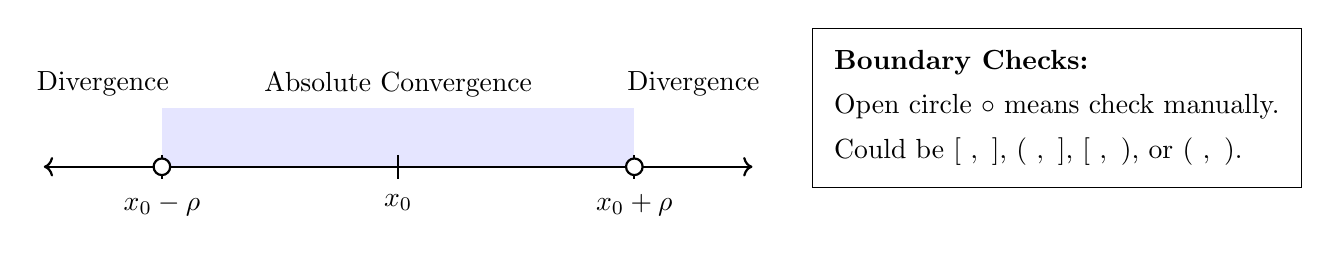
\begin{tikzpicture}[scale=1.5]
    % Background fill for convergence region
    \fill[blue!10] (1,0) rectangle (5,0.5);
    
    % Axis
    \draw[thick, <->] (0,0) -- (6,0);
    
    % Center and Radius
    \draw[thick] (3,0.1) -- (3,-0.1) node[below=2pt] {$x_0$};
    \draw[thick] (1,0.1) -- (1,-0.1) node[below=2pt] {$x_0 - \rho$};
    \draw[thick] (5,0.1) -- (5,-0.1) node[below=2pt] {$x_0 + \rho$};
    
    % Annotations
    \node[align=center, black] at (3, 0.7) {Absolute Convergence};
    \node[align=center, black] at (0.5, 0.7) {Divergence};
    \node[align=center, black] at (5.5, 0.7) {Divergence};
    
    % Boundary points
    \draw[fill=white, thick] (1,0) circle (2pt);
    \draw[fill=white, thick] (5,0) circle (2pt);
    
    % Legend
    \node[align=left, anchor=west, draw, inner sep=8pt] at (6.5, 0.5) {
        \textbf{Boundary Checks:}\\[4pt]
        Open circle $\circ$ means check manually.\\[4pt]
        Could be $[ \ , \ ]$, $( \ , \ ]$, $[ \ , \ )$, or $( \ , \ )$.
    };
\end{tikzpicture}
\end{center}

\subsection{Common Pitfalls and Traps}
\begin{itemize}
    \item \textbf{The Endpoint Trap:} The Ratio Test gives you the open interval $(x_0 - \rho, x_0 + \rho)$. It tells you \textit{nothing} about the endpoints. You MUST plug the endpoints back into the original series and use Calc II tests (like Alternating Series).
    \item \textbf{The Factorial Trap:} When doing the Ratio Test, remember that $(n+1)! = (n+1)n!$. A common mistake is writing $(2n+2)!$ as $2n!+2$. It is actually $(2n+2)(2n+1)(2n)!$.
    \item \textbf{The Integration Constant:} When integrating a power series to find a new function (like finding $\ln(1+x)$ from $\frac{1}{1+x}$), do not forget the $+ C$. You must solve for $C$ by plugging in the center point $x_0$.
\end{itemize}

\newpage
\section{Part 5: Conceptual Synthesis and The "Big Picture"}

\subsection{A) Thematic Connections}
The core theme of this chapter is \textbf{local approximation extending to global truth}. In Calculus I, we used the tangent line to approximate a function near a point (a 1st-degree Taylor polynomial). Power series take this to the infinite limit. By matching all infinitely many derivatives at a single point $x_0$, an analytic function's entire global behavior (within its radius of convergence) is perfectly encoded in that single local point. This is a profound philosophical result: for analytic functions, local data dictates global reality.

\subsection{B) Forward and Backward Links}
\textbf{Backward Links:} This topic relies heavily on the convergence tests from earlier in Calculus II. The Ratio Test is the engine of the power series. 
\textbf{Forward Links:} This chapter is the immediate prerequisite for solving Linear Differential Equations with variable coefficients (Section 8.3). When a differential equation like $y'' + xy' + y = 0$ cannot be solved with elementary functions, we assume the solution is a power series $y = \sum a_n x^n$, plug it in, shift indices, and solve for the coefficients $a_n$. Furthermore, Taylor series are the foundation of Complex Analysis (Laurent series) and numerical methods (Euler's method, Runge-Kutta).

\section{Part 6: Abstract Real-World Modeling (AI, ML, \& Quant Finance)}

\subsection{A) Concrete Scenarios}
1. \textbf{Quantitative Finance (The Greeks):} In options pricing, the Black-Scholes model provides a theoretical price for a derivative. Traders manage risk using "The Greeks" (Delta, Gamma, Theta), which are literally the coefficients of a multidimensional Taylor series expansion of the option's price with respect to underlying asset price and time.
2. \textbf{Machine Learning (Optimization):} Gradient Descent uses a first-order Taylor approximation of the loss function. Newton's Method for optimization uses a second-order Taylor polynomial (involving the Hessian matrix) to find the minimum of a loss function much faster by approximating the loss landscape as a series of parabolas.

\subsection{B) Model Problem Setup: Taylor Expansion in Risk Management}
Let $V(S, t)$ be the price of a European call option, where $S$ is the underlying stock price and $t$ is time. Suppose a quantitative hedge fund holds a portfolio of options. To hedge against small market movements $dS$ and time decay $dt$, the quant models the change in portfolio value $dV$ using a Taylor series expansion (which in stochastic calculus is formalized by It\^{o}'s Lemma):
\[ dV \approx \frac{\partial V}{\partial S} dS + \frac{\partial V}{\partial t} dt + \frac{1}{2} \frac{\partial^2 V}{\partial S^2} (dS)^2 \]
Here, the Taylor coefficients have specific financial names:
\begin{itemize}
    \item $\Delta = \frac{\partial V}{\partial S}$ (Delta: exposure to stock price)
    \item $\Theta = \frac{\partial V}{\partial t}$ (Theta: exposure to time decay)
    \item $\Gamma = \frac{\partial^2 V}{\partial S^2}$ (Gamma: convexity of the price curve)
\end{itemize}
To make the portfolio "Delta-Gamma neutral" (immune to both small and moderate stock price swings), the quant must solve a system of linear equations to balance the Taylor coefficients of the portfolio to zero, ensuring the series approximation of risk is strictly bounded.

\newpage
\section{Part 7: Common Variations and Untested Concepts}

\subsection{The Root Test for Radius of Convergence}
While the homework heavily emphasized the Ratio Test, the \textbf{Root Test} is sometimes necessary, especially when the $n$-th term is entirely raised to the $n$-th power.
\textbf{Theorem:} For $\sum a_n (x-x_0)^n$, let $L = \lim_{n \to \infty} \sqrt[n]{|a_n|}$. The radius of convergence is $\rho = \frac{1}{L}$.

\textbf{Example:} Find the radius of convergence for $\sum_{n=1}^{\infty} \left(\frac{2n+1}{n}\right)^n x^n$.
\\[6pt]
\textbf{Solution:} Applying the Root Test:
\[ L = \lim_{n \to \infty} \sqrt[n]{\left| \left(\frac{2n+1}{n}\right)^n \right|} = \lim_{n \to \infty} \frac{2n+1}{n} = 2 \]
Thus, the radius of convergence is $\rho = \frac{1}{2}$.

\subsection{Euler's Formula via Maclaurin Series}
A classic application of power series not covered in the exercises is proving Euler's formula: $e^{ix} = \cos x + i \sin x$.
By plugging $ix$ into the Maclaurin series for $e^x$:
\[ e^{ix} = \sum_{n=0}^{\infty} \frac{(ix)^n}{n!} = 1 + ix - \frac{x^2}{2!} - i\frac{x^3}{3!} + \frac{x^4}{4!} + i\frac{x^5}{5!} - \cdots \]
Grouping the real and imaginary parts perfectly yields the series for $\cos x$ and $\sin x$.

\section{Part 8: Advanced Diagnostic Testing: "Find the Flaw"}

Below are 5 problems with subtle errors. Act as the grader: find the flaw, explain it, and correct it.

\textbf{Problem 1:} Find the radius of convergence of $\sum_{n=1}^{\infty} \frac{(-1)^n x^n}{n}$.
\textit{Flawed Solution:} Let $a_n = \frac{(-1)^n}{n}$. $\lim \frac{a_{n+1}}{a_n} = \lim \frac{(-1)^{n+1}}{n+1} \frac{n}{(-1)^n} = \lim \frac{-n}{n+1} = -1$. Since the limit is $-1$, the radius is $\rho = -1$.
\\[6pt]
\textbf{Correction:} The flaw is forgetting the absolute value in the Ratio Test formula. The limit must be $\lim \left| \frac{a_{n+1}}{a_n} \right| = \lim \frac{n}{n+1} = 1$. The radius of convergence is strictly positive: $\rho = 1$.

\textbf{Problem 2:} Shift the index of $\sum_{n=2}^{\infty} a_n x^{n-1}$ so the generic term is $x^k$.
\textit{Flawed Solution:} Let $k = n-1$, so $n = k+1$. If $n=2$, then $k=1$. The new series is $\sum_{k=1}^{\infty} a_k x^k$.
\\[6pt]
\textbf{Correction:} The flaw is failing to substitute $n = k+1$ into the subscript of $a_n$. The correct series is $\sum_{k=1}^{\infty} a_{k+1} x^k$.

\textbf{Problem 3:} Find the Maclaurin series for $f(x) = \frac{1}{1+2x}$.
\textit{Flawed Solution:} We know $\frac{1}{1-x} = \sum x^n$. Substitute $2x$ for $x$ to get $\sum (2x)^n = \sum 2^n x^n$.
\\[6pt]
\textbf{Correction:} The flaw is a sign error. The denominator is $1 - (-2x)$. We must substitute $-2x$, yielding $\sum (-2x)^n = \sum (-1)^n 2^n x^n$.

\textbf{Problem 4:} Find the interval of convergence for $\sum_{n=1}^{\infty} \frac{x^n}{n^2}$.
\textit{Flawed Solution:} Ratio test gives $\rho = 1$. Endpoints are $x=1$ and $x=-1$. At $x=1$, $\sum \frac{1}{n^2}$ converges. At $x=-1$, $\sum \frac{(-1)^n}{n^2}$ diverges because it alternates. Interval is $( -1, 1 ]$.
\\[6pt]
\textbf{Correction:} The flaw is claiming the alternating series diverges. $\sum \frac{(-1)^n}{n^2}$ converges absolutely (and by the Alternating Series Test). The correct interval is $[ -1, 1 ]$.

\textbf{Problem 5:} Integrate $f(x) = \sum_{n=0}^{\infty} x^n$ to find the series for $-\ln(1-x)$.
\textit{Flawed Solution:} $\int \sum x^n dx = \sum_{n=0}^{\infty} \frac{x^{n+1}}{n+1}$. Therefore, $-\ln(1-x) = \sum_{n=0}^{\infty} \frac{x^{n+1}}{n+1}$.
\\[6pt]
\textbf{Correction:} The flaw is omitting the constant of integration $C$. While $C=0$ in this specific case (since $-\ln(1-0) = 0$), it must be explicitly stated and solved for: $-\ln(1-x) = C + \sum \frac{x^{n+1}}{n+1}$. Setting $x=0$ proves $C=0$.

\end{document}